\documentclass[a4paper,12pt]{article}
\usepackage{pdflscape}
\usepackage{fixltx2e}
\usepackage{textcomp}
\usepackage{fullpage}
\usepackage{float}
\usepackage{latexsym}
\usepackage{url}
\usepackage{epsfig}
\usepackage{graphicx}
\usepackage{amssymb}
\usepackage{amsmath}
\usepackage{bm}
\usepackage{array}
\usepackage[version=3]{mhchem}
\usepackage{ifthen}
\usepackage{caption}
\usepackage{hyperref}
\usepackage{amsthm}
\usepackage{amstext}
\usepackage{enumerate}
\usepackage[osf]{mathpazo}
\usepackage{dcolumn}
\usepackage{lineno}


\newcommand{\morphy}{\texttt{morphy} }

\begin{document}

%Running head
\begin{flushright}
Version dated: \today
\end{flushright}

\bigskip
\medskip
\begin{center}

\noindent{\Large \bf Description of \morphy library structures} 
\bigskip

\noindent {\normalsize \sc Martin Brazeau$^1$ and Thomas Guillerme$^1$}\\
\noindent {\small \it 
$^1$Imperial College London, Silwood Park Campus, Department of Life Sciences, Buckhurst Road, Ascot SL5 7PY, United Kingdom.}
\end{center}
% \medskip
% \noindent{*\bf Corresponding author.} \textit{guillert@tcd.ie}\\  
% \vspace{1in}

% %Line numbering
% \modulolinenumbers[1]
% \linenumbers


\section{\texttt{mfl\_node\_t}: Node structures}

The \texttt{mfl\_node\_t} are the structures that contain the phylogenetic information \textit{per se}: each can be a tip (\texttt{->nodet\_tip} $!= 0$ - e.g. node 0 in Fig.\ref{fig:Fig_tree_struct}) or a node (\texttt{->nodet\_tip} $== 0$ e.g. node 4 in Fig.\ref{fig:Fig_tree_struct}) and contain meta data such as the node/tip ID, name, position and character information.
Nodes are connect to each other either to form:
\begin{itemize}
    \item a \textbf{node ring}: where each \texttt{mfl\_node\_t} can be connected sequentially to each other to form a closed ring (via the \texttt{->nodet\_next} pointer).
    The rings next pointers can only point to a single node such as, for a node ring composed of three nodes, \texttt{node1->nodet\_next->nodet\_next->nodet\_next} points back to \texttt{node1} (e.g. the node ring formed of nodes 4, 5 and 9 in Fig.\ref{fig:Fig_tree_struct})
    \item an \textbf{edge}: where two different \texttt{mfl\_node\_t} can be connected to each other (via the \texttt{->nodet\_edge} pointer).
    In this case two nodes edges points to each other \texttt{node1->nodet\_edge} points to \texttt{node2} and \texttt{node2->nodet\_edge} points to \texttt{node1}.
    Note that \texttt{node1} and \texttt{node2} can be either tips (forming in that case a tree with only two taxa, one edge and zero nodes!) or nodes part of a node ring (e.g. node 0 (tip) and 7 (part of the ring) in Fig.\ref{fig:Fig_tree_struct}).
\end{itemize}

\section{\texttt{mfl\_tree\_t}: Tree structures}

The tree structure in \morphy are obtained by linking nodes (\texttt{mfl\_node\_t}) to each other via next (\texttt{->next}) and edge pointers (\texttt{->edge}).
The \texttt{mfl\_tree\_t} is composed of a node array (\texttt{mfl\_nodearray\_t}) containing the pointers to the nodes linked to each other, forming either node rings or tips.
The tree is also composed of metadata, namely the number of taxa and nodes or a pointer to the tree root (\texttt{mfl\_node\_t})).
Note that trees are can be rooted or not:
\begin{itemize}
    \item a \textbf{rooted} tree has it's \texttt{treet\_root} pointing to a \texttt{mfl\_node\_t}.
    In turn this \texttt{mfl\_node\_t} has an edge pointing to \texttt{NULL}.
    \item an \textbf{unrooted} tree has no \texttt{treet\_root} but a \texttt{treet\_start} pointing to any \texttt{mfl\_node\_t} in the tree.
\end{itemize}

\begin{figure}[!htbp]
\centering
    \includegraphics[keepaspectratio=true, width=0.8\textwidth]{Figures/tree_struct.pdf}
\caption{\texttt{mfl\_tree\_t} structure composed of connected \texttt{mfl\_node\_t} structures.}
\label{fig:Fig_tree_struct}
\end{figure}


\end{document}